\section{Unary Color Functions}
\label{sec:unary}

As discussed in Section~\ref{sec:approach}, color compatibility alone does not predict good pattern colorings. We observed that properties of a pattern region's color can depend on some key spatial features of that region. In this section, we define a set of color properties that we hypothesize contribute to good colorings, a set of spatial features that we use to predict distributions over those properties, and a general-purpose method for performing this prediction.

\subsection{Color Properties and Predictive Features}
\label{sec:unaryPropsAndFeatures}

While we could directly predict distributions over colors for pattern regions, predicting distributions instead over \emph{properties} of those colors (e.g. lightness or saturation) has benefits. First, it generalizes better to colors that do not occur in the training dataset but are consistent with that dataset's overall style: a training set that uses pastel colors might not contain a particular pastel blue, but that does not mean our system should not use it. Second, it allows the relative importance of different color properties to be tuned: it may be more critical to set the lightness of a pattern region correctly than to use the perfect hue. Similar approaches have been succesfully deployed to model the aesthetics of photographs~\cite{PhotoAesthetics}.

Many different color properties can contribute to the appearance of a pattern coloring. For the colors of individual pattern regions, our method considers the following set:
%%%
%\begin{description}[leftmargin=*]
\begin{description}
	\item[Lightness] is the L component of a color in the \lab color space. This value affects how bright the color appears to an observer.
	\item[Saturation] is the difference between a color and neutral gray, and affects how vivid the color appears. Rather than the typical HSV saturation, we use a more perceptually-based formula that operates in \lab space: $\frac{\sqrt{a^2+b^2}}{\sqrt{a^2+b^2+L^2}}$ ~\cite{ColorfulnessReference}.
	\item[Color Name Counts] is a vector of counts that summarizes how frequently a color is referred to using different names. The common names of a color often convey higher-level stylistic information about it. These vectors were derived in previous work from data collected in a large online color naming survey~\cite{ColorNamingModels}.
	\item[Color Name Saliency] is a measure of how reliably a color is named~\cite{ColorNamingModels}. It is derived through an entropy-based formulation and conveys information about how `instantly recognizable' a color is likely to be.
\end{description}
%%%
%
%\remark{Say something about how you could think of more properties, but we just decided to go with these ones for initial experimentation? and it's easy to add other properties into the model (but we already have some of this in the discussion section...)}
%
Distinctive spatial features of a color group, as well as the spatial features of the segments it contains, can affect the appearance of a color assignment. In our system, we use the following group features for color property prediction:
%%
\begin{description}
	\item[Relative Sizes] The area occupied by the group divided by the total area of the pattern, and the area divided by the maximum group area in the template.
  \item[Segment Spread] The 2D covariance matrix of the group's segment centroids. This feature captures whether the group is concentrated in one section of the pattern or spread across the whole pattern.
  \item[Segment Size Statistics] The minimum, maximum, mean, and standard deviation of the sizes of segments within the group.
  \item[Number of Segments] The number of segments in the group divided by the total number of segments in the image.
\end{description}
%%
We also consider the following features for individual segments within a color group:
%%
\begin{description}
	\item[Relative Sizes] The area occupied by the segment divided by the total area of the pattern, and the area divided by the maximum segment area in the template.
  \item[Normalized Discrete Compactness] A relationship between the segment's boundary edges and its area~\cite{NormalizedDiscreteCompactness}.
  \item[Elongation] The relative narrowness of a segment based on its minimum area bounding box: $1-\frac{\textrm{boxWidth}}{\textrm{boxHeight}}$. A square is the least elongated.
  \item[Centrality] Euclidean distance from the segment's centroid to the center of the pattern.
  \item[Role Labels] A set of three binary values: {\emph{Noise}, \emph{Background}, \emph{Foreground}}. \emph{Noise} indicates if the segment was labeled as `noise' during preprocessing (Section~\ref{sec:dataset}). \emph{Background} indicates if a segment belongs to the group with the largest connected component. All other segments are labeled \emph{Foreground}.
\end{description}

\subsection{Color Property Distributions}
\label{sec:unaryDistribs}

With a set of color properties and predictive spatial features in hand, our goal is to predict distributions over those properties given the features. Then, for a color group $\group$ and a color property $\prop$, we define the scoring function:
%%
\begin{equation*}
\groupInstStats(\colors_\group) =  \ln p( \prop( \colors_\group ) | \features_\group ) \cdot \size_\group
\end{equation*}
%%
where $\colors_\group$ is the color of group $\group$ and $\features_\group$ are its spatial features. We weight by the area of the group $\size_\group$ as larger regions tend to have more impact on the appearance of a coloring. Similarly, for a segment $\segment$, we define the function $\segInstStats(\colors_\segment) = \ln p( \prop( \colors_\segment ) | \features_\segment) \cdot \size_\segment$. Evaluating these functions on a particular color results in a `score' for how well that color fits the given group or segment, according to the property $\prop$.

Figure~\ref{fig:unaryHistograms} shows predicted distributions over lightness for different pattern regions using training data from the top 10 artists in our dataset. The background color group, which is larger and more spread, exhibits a bimodal distribution. Intuitively, backgrounds are either dark or light but rarely of middling brightness. The distribution favors light backgrounds, reflecting the stylistic biases of the data used for training. The smaller, more concentrated, foreground flower color group, on the other hand, strictly prefers lighter colors.

\begin{figure}[ht]
\centering
\begin{tabular}{cc}
{\raisebox{2.5em}{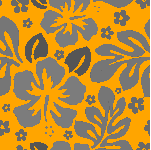
\includegraphics[width=.25\columnwidth]{figs/histograms/b}}}&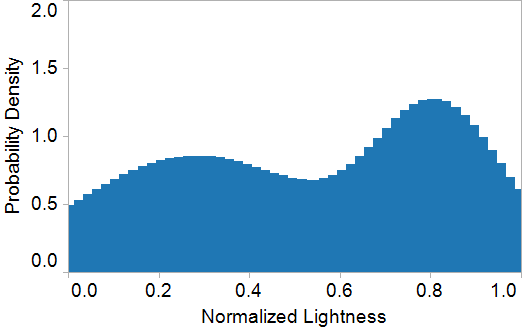
\includegraphics[width=.60\columnwidth]{figs/histograms/backgroundGroupHistogram-small}\vspace{0.5em}\\
{\raisebox{2.5em}{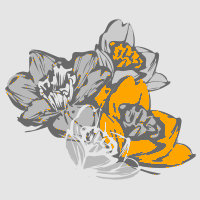
\includegraphics[width=.25\columnwidth]{figs/histograms/f}}}&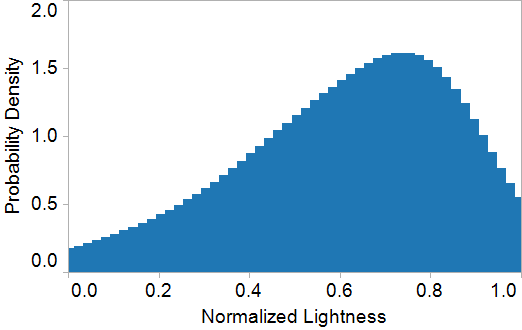
\includegraphics[width=.60\columnwidth]{figs/histograms/foregroundGroupHistogram-small}\vspace{0.5em}\\
\end{tabular}

\caption{Predicted distributions over lightness for two different color groups (higlighted in orange). The background has a bimodal distribution, whereas the foreground strictly favors lighter colors.}
\label{fig:unaryHistograms}
\vspace{-1.0em}
\end{figure}

How should we represent these distributions $p$? Closed-form continuous distributions, such as the normal distribution, are appealing for their simplicity.  However, they are unlikely to capture the shape of distributions exhibited by real patterns, which are often \emph{multimodal} in nature (Figure~\ref{fig:unaryHistograms}).

%, who build multimodal distributions of colors given local texture features for grayscale image colorization.
We adapt the method of Charpiat et al.~\shortcite{MultimodalColorization} to build multimodal distributions of color properties. We first discretize the space of possible color property values into a finite number of bins. Next, we train a multi-class classifier on $(\prop(\colors), \features)$ pairs extracted from the training dataset. This classifier predicts, given a feature vector $\features$, the probability that its corresponding property value $\prop(\colors)$ falls into each bin. Given a never-before-seen feature vector, the classifier can then output a \emph{histogram} of these probabilities, one for each property value bin. The histogram is then smoothed using kernel density estimation, and the resulting density forms the final, continuous probability distribution.

In our implementation, we discretize the space of property values using K-means clustering with $k = 10$ on the values found in the training examples. We then use multinomial logistic regression to predict the histograms of color property values given features.
%To ensure each pattern template in the training set has equal influence in the regression, we weight each group example by one over the number of groups in the template; segment examples are weighted similarly.
Finally, we smooth the histograms by placing a Gaussian at the center of each histogram bin and setting the Gaussian bandwidth to the average distance to the nearest three other bins~\cite{ThemeEnhancement}.